\documentclass{ximera}
\input{preamble}
\input{orccaImagePreamble}
\usepackage{hyperref}
\usepackage{lipsum}
\usepackage{lmodern}
\usepackage{tcolorbox}



\author{Elizabeth Miller}
\license{Creative Commons 4.0 International License}
\acknowledgement{https://spot.pcc.edu/math/orcca/ed2/html/orcca.html}


\title{Relations and Graphs: Cartesian Coordinates}

\begin{document}

\begin{abstract}
We graph points on a 2-dimensional Cartesian graph.  %We define relations and graph examples of examples.  We also list important relations that will be explored throughout this course and used often in Calculus.
\end{abstract}
\maketitle

%\typeout{************************************************}
%\typeout{Graphing 2-D Cartesian Coordinates}
%\typeout{************************************************}

\section{Graphing 2-D Cartesian Coordinates} 
% From https://spot.pcc.edu/math/orcca/ed2/html/section-cartesian-coordinates.html 

When we model a relationship between two variables visually, we use the Cartesian coordinate system. We begin with the basic vocabulary and ideas that come with the Cartesian coordinate system.

The Cartesian coordinate system identifies the location of every point in a plane. Basically, the system gives every point in a plane its own “address” in relation to a starting point. We'll use a street grid as an analogy. Here is a map with Carl's home at the center. The map also shows some nearby businesses. Assume each unit in the grid represents one city block.

\begin{tikzpicture}
    \begin{axis}[xlabel={},ylabel={},width=0.47\linewidth,
                xmin=-5,xmax=5,
                ymin=-5,ymax=5,
                xtick={-4,4},
                ytick={-4,4},
                clip=false]
        \addplot[soliddot] coordinates {(0,0)} node[pin=240:{Carl's house}] {};
        \addplot[soliddot] coordinates {(2, 3)} node[pin=-30:{restaurant}] {};
        \addplot[soliddot] coordinates {(-3, 2)} node[pin=100:{pet shop}] {};
        \addplot[soliddot] coordinates {(-2, -4)} node[pin=150:{gas station}] {};
        \addplot[soliddot] coordinates {(3, -3)} node[pin=120:{bar}] {};
        \addplot[mark=none] coordinates {(5, 0)} node[above left] {east};
        \addplot[mark=none] coordinates {(-5, 0)} node[above right] {west};
        \addplot[mark=none] coordinates {(0, 5)} node[below right] {north};
        \addplot[mark=none] coordinates {(0, -5)} node[above right] {south};
    \end{axis}
\end{tikzpicture}

If Carl has an out-of-town guest who asks him how to get to the restaurant, Carl could say, “First go 2 blocks east (to the right on the map), then go 3 blocks north (up on the map).”

Two numbers are used to locate the restaurant. In the Cartesian coordinate system, these numbers are called coordinates and they are written as the ordered pair (2,3). The first coordinate, 2, represents distance traveled from Carl's house to the east (or to the right horizontally on the graph). The second coordinate, 3, represents distance to the north (up vertically on the graph).

\begin{tikzpicture}
    \begin{axis}[xlabel={},ylabel={},
                xmin=-5,xmax=5,
                ymin=-5,ymax=5,
                xtick={-4,4},
                ytick={-4,4},
                clip=false]
        \addplot[soliddot] coordinates {(0,0)} node[pin=240:{Carl's house}] {};
        \addplot[soliddot] coordinates {(2, 3)} node[pin=-30:{restaurant}] {} node[left] {$(2,3)$};
        \addplot[soliddot,opacity=0] coordinates {(-2, -4)} node[pin=150:{gas station}] {};
        \addplot[mark=none] coordinates {(5, 0)} node[above left] {east};
        \addplot[mark=none] coordinates {(-5, 0)} node[above right] {west};
        \addplot[mark=none] coordinates {(0, 5)} node[below right] {north};
        \addplot[mark=none] coordinates {(0, -5)} node[above right] {south};
        \addplot[firstcurve,-] coordinates {(0,0) (2,0)} node[below,pos=0.5] {right $2$};
        \addplot[firstcurve,->] coordinates {(2,0) (2,2.8)} node[below,pos=0.5,rotate=90] {up $3$};
    \end{axis}
\end{tikzpicture}

To travel from Carl's home to the pet shop, he would go 3 blocks west, and then 2 blocks north.

In the Cartesian coordinate system, the positive directions are to the right horizontally and up vertically. The negative directions are to the left horizontally and down vertically. So the pet shop's Cartesian coordinates are $(-3,2)$.

\begin{tikzpicture}
    \begin{axis}[xlabel={},ylabel={},
                xmin=-5,xmax=5,
                ymin=-5,ymax=5,
                xtick={-4,4},
                ytick={-4,4},
                clip=false]
        \addplot[soliddot] coordinates {(0,0)} node[pin=240:{Carl's house}] {};
        \addplot[soliddot] coordinates {(-3, 2)} node[pin=100:{pet shop}] {} node[above right] {$(-3,2)$};
        \addplot[soliddot,opacity=0] coordinates {(-2, -4)} node[pin=150:{gas station}] {};
        \addplot[soliddot,opacity=0] coordinates {(2, 3)} node[pin=-30:{restaurant}] {};
        \addplot[mark=none] coordinates {(5, 0)} node[above left] {east};
        \addplot[mark=none] coordinates {(-5, 0)} node[above right] {west};
        \addplot[mark=none] coordinates {(0, 5)} node[below right] {north};
        \addplot[mark=none] coordinates {(0, -5)} node[above right] {south};
        \addplot[firstcurve,-] coordinates {(0,0) (-3,0)} node[below,pos=0.5] {left $3$};
        \addplot[firstcurve,->] coordinates {(-3,0) (-3,1.8)} node[below,pos=0.5,rotate=90] {up $2$};
    \end{axis}
\end{tikzpicture}


\begin{tcolorbox}[colback=blue!5]
\begin{remark}
 It's important to know that the order of Cartesian coordinates is (horizontal, vertical). This idea of communicating horizontal information before vertical information is consistent throughout most of mathematics.
\end{remark}
\end{tcolorbox}

\begin{example}[Check Your Understanding]
Use the graph above about Carl's neighborhood to answer the following questions.
\begin{itemize}
\item What are the coordinates of the bar? $\answer{(3,-3)}$
\item What are the coordinates of the gas station? $\answer{(-2,-4)}$
\item What are the coordinates of Carl's house? $\answer{(0,0)}$
\end{itemize}
\end{example}

\begin{tcolorbox}[colback=blue!5]
\begin{remark}[Notation Issue]
Unfortunately, the notation for an ordered pair looks exactly like interval notation for an open interval. Context will help you understand if (1,3) indicates the point 1 unit right of the origin and 3 units up,

\begin{tikzpicture}
    \begin{axis}[xlabel={},ylabel={},width=1.625in,
                xmin=-5,xmax=5,
                ymin=-5,ymax=5,
                xtick={-4,4},
                ytick={-4,4},
                clip=false]
        \addplot[soliddot] coordinates {(1, 3)} node[right] {$(1,3)$};
    \end{axis}
\end{tikzpicture}

 or if (1,3) indicates the interval of all real numbers between 1 and 3.

\begin{tikzpicture}
    \begin{axis}[numberline,width=1.625in,
                xmin=-5,xmax=5,
                xtick={1,3},
                ]
        \addplot[openinterval] coordinates {(1,0) (3,0)} node[pos=0.5,above] {$(1,3)$};
    \end{axis}
\end{tikzpicture}
\end{remark}
\end{tcolorbox}

Traditionally, the variable $x$ represents numbers on the horizontal axis, so it is called the $x$-axis. The variable $y$ represents numbers on the vertical axis, so it is called the $y$-axis.  The axes meet at the point $(0,0)$, which is called the origin. Every point in the plane is represented by an ordered pair, $(x,y)$.  

In a Cartesian coordinate system, the map of Carl's neighborhood would look like this:

\begin{tikzpicture}
    \begin{axis}[xmin=-5,xmax=5,width=0.47\linewidth,
                ymin=-5,ymax=5,
                xtick={-4,4},
                ytick={-4,4}]
        \addplot[soliddot] coordinates {(0,0)} node[above right] {(0,0)};
        \addplot[soliddot] coordinates {(2, 3)} node[above] {(2,3)};
        \addplot[soliddot] coordinates {(-3, 2)} node[above] {(-3,2)};
        \addplot[soliddot] coordinates {(-2, -4)} node[above] {(-2,-4)};
        \addplot[soliddot] coordinates {(3, -3)} node[above] {(3,-3)};
    \end{axis}
\end{tikzpicture}

\begin{tcolorbox}
\begin{definition}
The \textbf{Cartesian coordinate system} is a coordinate system that specifies each point uniquely in a plane by a pair of numerical coordinates, which are the signed (positive/negative) distances to the point from two fixed perpendicular directed lines, measured in the same unit of length. Those two reference lines are called the \textbf{horizontal axis} and \textbf{vertical axis}, and the point where they meet is the \textbf{origin}. The horizontal and vertical axes are often called the \textbf{$x$-axis} and \textbf{$y$-axis}.  \\

The plane based on the $x$-axis and $y$-axis is called a \textbf{coordinate plane}. The ordered pair used to locate a point is called the point's \textbf{coordinates}, which consists of an $x$-coordinate and a $y$-coordinate. For example, the point $(1,2)$, has $x$-coordinate 1,  and $y$-coordinate 2.   The origin has coordinates $(0,0)$. \\

A Cartesian coordinate system is divided into four \textbf{quadrants}, as shown below . The quadrants are traditionally labeled with Roman numerals.

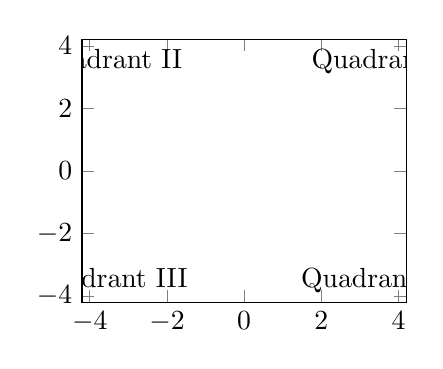
\begin{tikzpicture}
    \begin{axis}[width=0.47\linewidth]
        \addplot[mark=none] coordinates {(3.5,3.5)} node[] {Quadrant I};
        \addplot[mark=none] coordinates {(-3.5, 3.5)} node[] {Quadrant II};
        \addplot[mark=none] coordinates {(-3.5, -3.5)} node[] {Quadrant III};
        \addplot[mark=none] coordinates {(3.5, -3.5)} node[] {Quadrant IV};
    \end{axis}
\end{tikzpicture}

\end{definition}
\end{tcolorbox}

\begin{example}
On paper, sketch a Cartesian coordinate system with units, and then plot the following points: $(3,2)$, $(-5,-1)$, $(0,-3)$, $(4,0)$.

\begin{solution} 

\begin{tikzpicture}
    \begin{axis}[]
        \addplot[soliddot] coordinates {(3, 2)} node[above] {$(3,2)$};
        \addplot[soliddot] coordinates {(-5, -1)} node[below] {$(-5,-1)$};
        \addplot[soliddot] coordinates {(0, -3)} node[right] {$(0,-3)$};
        \addplot[soliddot] coordinates {(4, 0)} node[above] {$(4,0)$};
    \end{axis}
\end{tikzpicture}
\end{solution}
\end{example}


\end{document}
